\documentclass[a4paper]{article}

\usepackage[utf8]{inputenc}
\usepackage{graphicx}

\parindent 0px

\title{Das Epische Theater}
\author{Alin Porcic}

\begin{document}

	\maketitle

	\newpage
	\section{Das Epische Theater}

        Das Epische Theater, Begriff von Bertolt Brecht geprägt, verbindet die zwei literarische Gattungen: die Dramatik und die Epik. Im den 1920er Jahren experimentierten Bertholt Brecht und Erwin Piscator und versuchten die Darstellung der tragischen Einzelschicksale zu vermeiden. Das Ziel war es große gesellschaftliche Konflikte, wie zum Beispiel Kriege, Revolutionen oder soziale Ungerechtigkeit, durchschaubar zu machen und den Zuseher dazu bewegen, die Gesellschaft zum Positiven zu verändern.\\\\

        Der Zuschauer soll das Geschehen kritisch und emotionslos Betrachten und sich dabei von den Ereignissen distanzieren. Das Mitgefühl der Zuschauer zu den Figuren soll unterbunden werden und der Zuschauer soll gesellschaftliche Erkenntnisse sammeln. Im Gegensatz zum aristotelischen Theater hat das Epische Theater keinen Spannungbogen, jede Szene steht für sich und kann in der Reihenfolge verändert werden. Ein offener Schluss ist im Epischen Theater eher üblich.\\\\

	Die Verfremdungseffekte sind stilistische Methoden, die das Epische Theater anwendet, um die Entstehung von Spannung zu vermeiden. Die Spannung verhindert den Zuschauer im Denken und Lernen, daher muss die Spannung schon vor der Aufführung der Szenene entfernt werden. Das geschieht durch folgende Methoden:
        
        \begin{itemize}
	\item Der Szeneninhalt wird schon vor der Aufführung der jeweiligen Szenen erzählt. Damit weiß der Zuschauer was ihm erwartet und er kann sich ganz auf den Inhalt des Stücks konzentieren.
        \item Das Bühnenbild wird gezielt verändert, sodass der Zuschauer immer weiß, dass er sich im Theater befindet und die Ereignisse nicht real sind.
        \item Kommentare unterbrechen die Handlungen, Figuren treten aus ihren Rollen aus und wenden sich an das Publikum
        \item Es wird zum Teil in Versen gesprochen.
        \item Die Schauspieler selbst bauen eine Distanz zur gespielten Figur auf, damit die Zuschauer den Protagonisten nicht als Identifikationsfigur wahrnehmen können. Die Figuren können kritische betrachtet werden.
        \end{itemize}
        
        \newpage
        \section{Bertolt Brecht (1898 - 1956)}

	Bertolt Brecht wurde am 10.Febuar 1898 in Augsburg, Deutschland, geboren und wuchs in gesicherten ökonomischen und sozialen Verhältnissen auf. Sein Vater hatte keine höhere Schulausbildung, konnte sich aber in der Augsburger Haindl'schen Papierfabrik zum Direktor hoch arbeiten.\\\\
        Bertolt Brecht besuchte stadesgemäß das Realgymnasium und brachte regelmäßig gute, wenn nicht sehr gute Zeugnisse nach Hause.\\\\
        Schon im jungen Alter began Bertolt mit dem Dichten und arbeitet zusammen mit seinen Freunden an einer Schülerzeitung. Er verfasste Gedichte, Prosatexte und sogar ein einaktiges Drama, die Bibel. In den folgenden Jahren produzierte er weitere Gedichte und Dramenentwürfe.\\\\
        Nach dem Beginn des Ersten Weltkrieges 1914 gelang es ihm, eine Serie von Reportagen und Rezensionen in die lokalen und reginalen Medien unterzubringen (München-Augsburger Abendzeitung). 1916 verfasste er Gedichte, die in der späteren Sammlung 'Bertolt Brechts Hauspostille' eingebunden wurden.\\\\
             
       	\section{Nennenswerte Autoren und Werke}
	        
        \section{Mutter Courage und ihre Kinder}

	'Mutter Courage und ihre Kinder' ist ein Drama, welches von Bertolt Brecht im schwedischen Exil 1938/39 verfasst wurde und 1941 in Zürich uraufgeführt wurde.
        
	\subsection{Inhaltsangabe}


        
        \subsection{Figurenkonstallation}
	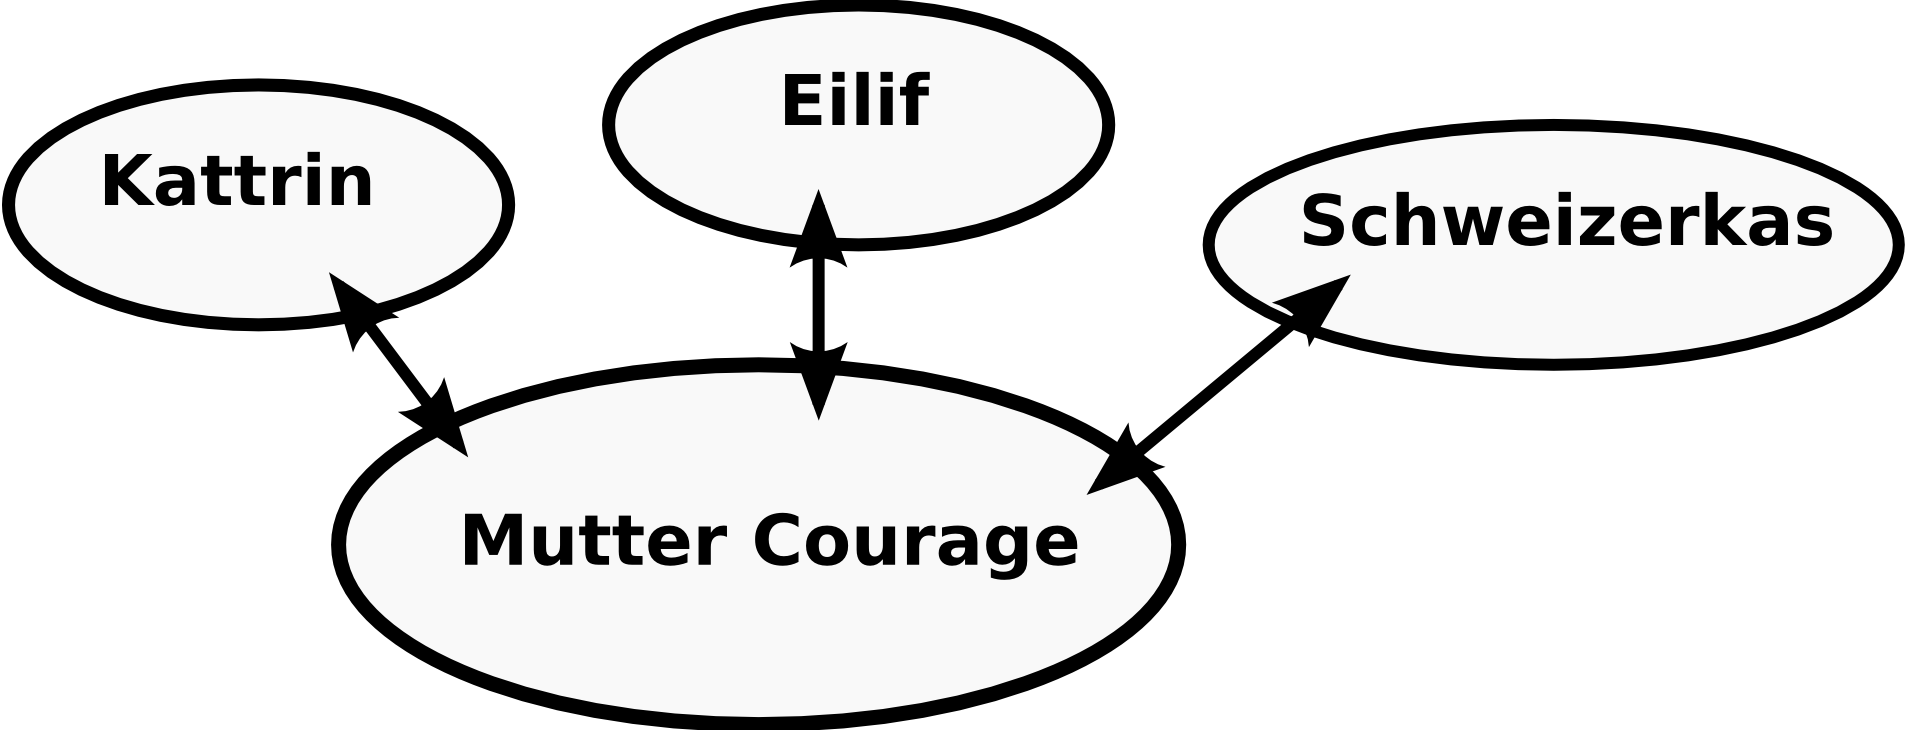
\includegraphics[width=250px]{img/figuren.png}

        
\end{document}
